\begin{refsection}
\chapter{Appendix B} % Main chapter title
\label{appendix_B}


\section*{The biologically-constrained feasibility domain, $\beta$}
We used Monte-Carlo integration methods to estimate the size of the biologically-constrained feasibility domain ($\beta$); that is, the area where both species can have positive abundances given competitive, abundance, and model-based constraints. We performed this integration on the growth-rate parameter space. First, we determined the maximum possible value of the radius ($R$) to integrate over given the abundance constraints under consideration. To do this, we first defined a radius $R$,  as a function of both species' intrinsic growth rates:
\begin{equation}
  R = \sqrt{r_{i}^{2} + r_{j}^{2}} \,,
\end{equation}
where  $r_{i}$ and $r_{j}$ are the growth rates of species $i$ and $j$ defined by each model, respectively. We know that, for all of the models used, the vector of species growth rates can be expressed as a linear function of species densities such that:
\begin{equation}
\begin{bmatrix}
r_{i} \\
r_{j}
\end{bmatrix} =
\begin{bmatrix}
\alpha_{ii} & \alpha_{ij} \\
\alpha_{ji} & \alpha_{jj}
\end{bmatrix}
\begin{bmatrix}
g_{i}N_{i}^{*}\\ g_{j}N_{j}^{*}
\end{bmatrix} \,,
\end{equation}
where the elements of the interaction matrix denote the change in per capita growth rate of species $i$ under a small change in the density of species $j$, and $g_{i}N_{i}^{*}$ and $g_{j}N_{j}^{*}$ define the vector of abundances for species $i$ and $j$. Species growth rates can therefore be expressed as:
\begin{eqnarray}
  r_{i} = \alpha_{ii}g_{i}N_{i}^{*} + \alpha_{ij}g_{j}N_{j}^{*}\\
  r_{j} = \alpha_{ji}g_{i}N_{i}^{*} +\alpha_{jj}g_{j}N_{j}^{*}
\end{eqnarray}

We must therefore find the maximum value of R given constraints on the maximum abundance of species $i$ ($g_{i}N_{i,max}^{*}$) and of species $j$ ($g_{j}N_{j,max}^{*}$). In the following sections, we show 9 scenarios that describe all the possible values $R$ can take under such constraints, and how to determine if they can be a maximum.

\subsection*{Scenario 1: Both species are absent}

If both $g_{i}N_{i}^{*}$ and $g_{j}N_{j}^{*}$ have a value of zero, then $R = 0$.

\subsection*{Scenario 2: Species $i$ is at its maximum abundance and species $j$ is absent}

Then, the value of $R$ is:
\begin{equation}
R = \sqrt{ (\alpha_{ii}g_{i}N_{i,max}^{*})^{2} + (\alpha_{ji}g_{i}N_{i,max}^{*})^{2} }.
\label{scenario2}
\end{equation}

\subsection*{Scenario 3: Species $i$ is absent and species $j$ is at its maximum abundance}

Then the value of $R$ is:
\begin{equation}
R = \sqrt{ (\alpha_{ij}g_{j}N_{j,max}^{*})^{2} + (\alpha_{jj}g_{j}N_{j,max}^{*})^{2} }.
\label{scenario3}
\end{equation}


\subsection*{Scenario 4: Both species are at their maximum abundance}
If both species are at their maximum abundance then:
\begin{equation}
\label{scenario4}
R = \sqrt{ (\alpha_{ii}g_{i}N_{i,max}^{*} +\alpha_{ij}g_{j}N_{j,max}^{*})^{2} + ( \alpha_{ji}g_{i}N_{i,max}^{*}+ \alpha_{jj}g_{j}N_{j,max}^{*})^{2} }.
\end{equation}

\subsection*{Scenario 5: Species $j$ is absent }

%DBS: The below is not looking for fixed points. It should be looking for maxima. We need to rephrase.
When species $j$ is absent, then:
\begin{equation}
  R = \sqrt{ (\alpha_{ii}g_{i}N_{i}^{*})^{2} + (\alpha_{ji}g_{i}N_{i}^{*})^{2}  }
\end{equation}
To find the maximum, for mathematical simplicity we can differentiate $R^{2}$:
\begin{equation}
  \frac{\partial R^{2}}{\partial g_{i}N_{i}^{*}} = \alpha_{ii}^{2}2g_{i}N_{i}^{*} + \alpha_{ji}^{2}2g_{i}N_{i}^{*} \,,
\end{equation}
and the value of $g_{i}N_{i}^{*}$ that corresponds to a maximum:
\begin{eqnarray}
  \alpha_{ii}^{2}2g_{i}N_{i}^{*} + \alpha_{ji}^{2}2g_{i}N_{i}^{*}  = 0 \\
  g_{i}N_{i}^{*} (2\alpha_{ii}^{2} +  2\alpha_{ji}^{2}) = 0 \\
  g_{i}N_{i}^{*}= 0
\end{eqnarray}
which inevitably implies $R = 0$. Thus when species $j$ is absent, the maximum of $R$ is at cero and the maximum value of $R$ is at the boundary of the constraints.



\subsection*{Scenario 6: Species $i$ is absent }
By symmetry, when species $i$ is absent, the maximum value of $R$ is  at the boundary of the constraints.

\subsection*{Scenario 7: Species $j$ is at its maximum abundance }
We can redefine $R^{2}$ as:
\begin{equation}
   R^2 = (\alpha_{ii}g_{i}N_{i}^{*} + \alpha_{ij}g_{j}N_{j,max}^{*} )^2 + (\alpha_{ji}g_{i}N_{i}^{*} + \alpha_{jj}g_{j}N_{j,max}^{*} )^2 \,,
\end{equation}
and find the value of $g_{i}N_{i}^{*}$ where there is a maixmum of $R$:
\begin{eqnarray}
  \frac{\partial R^{2}}{\partial g_{i}N_{i}^{*}}= 0 = \alpha_{ii}^{2}2g_{i}N_{i}^{*}  +2\alpha_{ii}\alpha_{ij}g_{j}N_{j,max}^{*} +  \alpha_{ji}^{2}2g_{i}N_{i}^{*} + 2\alpha_{ji}\alpha_{jj}g_{j}N_{j,max}^{*}\\
  g_{i}N_{i}^{*} = \frac{- \alpha_{ii}\alpha_{ij}g_{j}N_{j,max}^{*} - \alpha_{ji}\alpha_{jj}g_{j}N_{j,max}^{*}}{\alpha_{ii}^2 + \alpha_{ji}^2} \,.
\end{eqnarray}
Then the value of $R$ that corresponds to this scenario is:

\begin{equation}
  R = \sqrt{
\begin{aligned}
  ((\frac{- \alpha_{ii}\alpha_{ij}g_{j}N_{j,max}^{*} - \alpha_{ji}\alpha_{jj}g_{j}N_{j}^{*}}{\alpha_{ii}^2 + \alpha_{ji}^2}\alpha_{ii} + \alpha_{ij}g_{j}N_{j,max}^{*} )^2 \\
  + (\frac{- \alpha_{ii}\alpha_{ij}g_{j}N_{j,max}^{*} - \alpha_{ji}\alpha_{jj}g_{j}N_{j,max}^{*}}{\alpha_{ii}^2 + \alpha_{ji}^2}\alpha_{ji} + \alpha_{jj}g_{j}N_{j,max}^{*} )^2
\end{aligned}
}
\label{scenario7}
\end{equation}

%+ (\frac{- \alpha_{ii}\alpha_{ij}g_{j}N_{j,max}^{*} - \alpha_{ji}\alpha_{jj}g_{j}N_{j,max}^{*}}{\alpha_{ii}^2 + \alpha_{ji}^2}\alpha_{ji} + \alpha_{jj}g_{j}N_{j,max}^{*} )^2


\subsection*{Scenario 8: Species $i$ is at its maximum abundance}

Similar to the previous scenario, the value of $R$ that corresponds to this scenario is:


\begin{equation}
  R = \sqrt{
\begin{aligned}
  (\alpha_{ii}g_{i}N_{i,max}^{*} + \frac{-\alpha_{ii}\alpha_{ij}g_{i}N_{i,max}^{*} - \alpha_{ji}\alpha_{jj}g_{i}N_{i,max}^{*}}{\alpha_{ij}^{2} + \alpha_{jj}^{2}}\alpha_{ij} )^2 \\
  + (\alpha_{ji}g_{i}N_{i,max}^{*} + \frac{-\alpha_{ii}\alpha_{ij}g_{i}N_{i,max}^{*} - \alpha_{ji}\alpha_{jj}g_{i}N_{i,max}^{*}}{\alpha_{ij}^{2} + \alpha_{jj}^{2}}\alpha_{jj} )^2
\end{aligned}
}
\label{scenario8}
\end{equation}


\subsection*{Scenario 9: Neither species is at its maximum abundance}

If both species are present but neither of is at their maximum abundances, then:
\begin{equation}
  R^{2} =  (\alpha_{ii}g_{i}N_{i}^{*} + \alpha_{ij}g_{j}N_{j}^{*}) ^{2} + (\alpha_{ji}g_{i}N_{i}^{*} +\alpha_{jj}g_{j}N_{j}^{*})^{2} \,
\end{equation}
which can be expanded to:

\begin{equation}
\label{R2expanded}
R^{2} =  \alpha_{ii}^{2}g_{i}N_{i}^{*2} + 2 \alpha_{ii}\alpha_{ij}g_{i}N_{i}^{*}g_{j}N_{j}^{*} +\alpha_{ij}^{2} g_{j}N_{j}^{*2} +\alpha_{ji}^{2} g_{i}N_{i}^{*2}
+  2 \alpha_{ji}\alpha_{jj}g_{i}N_{i}^{*}g_{j}N_{j}^{*}  + \alpha_{jj}^{2} g_{j}N_{j}^{*2}
\end{equation}

To find a maximum, we require:
\begin{eqnarray}
  \frac{\partial R_{2}}{\partial g_{i}N_{i}^{*}} = \alpha_{ii}^{2}2g_{i}N_{i}^{*} + 2\alpha_{ii}\alpha_{ij}g_{j}N_{j}^{*} + \alpha_{ji}^{2}2g_{i}N_{i}^{*} + 2\alpha_{ji}\alpha_{jj}g_{j}N_{j}^{*}\\
\frac{\partial R_{2}}{\partial g_{j}N_{j}^{*}}  = 2\alpha_{ii}\alpha_{ij}g_{i}N_{i}^{*} + \alpha_{ij}^{2}2g_{j}N_{j}^{*} + 2\alpha_{ji}\alpha_{jj} g_{i}N_{i}^{*} + \alpha_{jj}^{2}2g_{j}N_{j}^{*}
\end{eqnarray}

If we solve for the abundance of species $i$ in the second equation at a maximum:
\begin{eqnarray}
 \alpha_{ii}\alpha_{ij}g_{i}N_{i}^{*} + \alpha_{ij}^{2}g_{j}N_{j}^{*} + \alpha_{ji}\alpha_{jj}g_{i}N_{i}^{*} + \alpha_{jj}^{2}g_{j}N_{j}^{*}= 0 \\
  N{i} = - g_{j}N_{j}^{*}\frac{\alpha_{ij}^{2} + \alpha_{jj}^{2}}{ \alpha_{ii}\alpha_{ij} + \alpha_{ji}\alpha_{jj}}
\end{eqnarray}
and for species $j$ in the first equation:
\begin{eqnarray}
 \alpha_{ii}^{2}- g_{j}N_{j}^{*}\frac{\alpha_{ij}^{2} + \alpha_{jj}^{2}}{ \alpha_{ii}\alpha_{ij} + \alpha_{ji}\alpha_{jj}} + \alpha_{ii}\alpha_{ij}g_{j}N_{j}^{*} + \alpha_{ji}^{2}- g_{j}N_{j}^{*}\frac{\alpha_{ij}^{2} + \alpha_{jj}^{2}}{ \alpha_{ii}\alpha_{ij} + \alpha_{ji}\alpha_{jj}} + \alpha_{ji}\alpha_{jj}g_{j}N_{j}^{*} = 0\\
g_{j}N_{j}^{*} = 0
\end{eqnarray}

This implies that there is no maximum for when both species are present but neither of them is at their maximum abundance. As a result of these nine scenarios, the maximum value of $R$ can be found only where one or both of the species are at their maximum abundances, which correspond to only five possible scenarios (Eqns.~\ref{scenario2} \ref{scenario3}, \ref{scenario4}, \ref{scenario7}, \ref{scenario8}). In our framework, given an interaction matrix and the constraints on species abundances, we calculated the value of $R$ for each one of the five possible scenarios and chose the value that was the highest.



\subsection*{Integration methods}

Once we determined the range of $R$ to integrate over, we performed a Monte Carlo Integration to determine the size of the biologically-constrained feasibility domain. We did this by generating random points within a circle of radius $R$. We discarded points that did not correspond to positive abundances of both species given their interaction matrix (i.e., we kept only feasible growth rates). We further discarded points that corresponded to abundances greater than $g_{i}N_{i,max}^{*}$ and $g_{j}N_{j,max}^{*}$. Finally, we discarded all of the points that fell outside the model-based constraints for each species (Table 1 of the main text). This method allowed us to sample points that were feasible \textit{and} biologically plausible. We set our integration to sample random points until we had at least 500 points inside the feasible and biologically-plausible space, or when it reached 200,000 total samples. We also kept track of all of the points that were discarded. All calculations were done in the programming language \textit{R} \citep{Rcore}.


Once we had a sample of feasible and biologically plausible points, we determined the points that comprise the convex hull around them using the function \textit{chull} from the package \textit{grDevices}. To determine the vertices of the convex hull, we required a sample of at least 4 points. If the sample of the MC integration was lower than 4 points, we did not perform further calculations and determined that the biologically-constrained feasibility domain could not be detected and was effectively of size $\beta \approx 0$. To determine if the vertices were in fact describing a convex hull, we also kept track if any of the discarded points could be inside the area described by the vertices using the function \textit{point.in.polygon} from the package \textit{sp}. Finally, we determined the size of the area described by the convex hull using the function \textit{Polygon} from the package \textit{sp}.
%NUMBER of vertices varies
% DBS: Since the bit below depends on us having many vertices, do we need to say how the above determines the granularity of the convex hull's boundary?



\section*{Minimum distance from the edge, $\delta$}

To calculate the minimum euclidean distance from the observed growth rates to the edge of the biologically-constrained feasibility domain, we used the set of vertices describing that domain's boundaries. For every two adjacent vertices, we calculated the distance between species' growth rates $r_{i}$ and $r_{j}$, and the perpendicular projection of the line between the vertices using the function \textit{pointLineD} from the package \textit{SpatialGraph}. We also calculated the euclidean distance between the observed growth rates and the two adjacent vertices. From those three measures, we determined the shortest distance. We performed these calculations for every set of adjacent vertices, and determined $\delta$ as the minimum of all of the values we obtained.


\section*{Area in monoculture, $\gamma$}

% DBS: I don't understand what $r_{i,c}$ etc corresponds to.
% DBS: Oh wait. Aren't we neglecting to mention that $0,0$ is always a corner of this space?
To determine the parameter space where both species can grow in monoculture given abundance and model-based constraints, we first determined the constrained values of species growth rates $r_{i,c}$ and $r_{j,c}$. Note that empirical values of species growth rates $r_{i}$ and $r_{j}$ can take negative values if competition coefficients are negative, which would imply facilitative interactions. Necesarily, the parameter space where both species can grow in monoculture includes the coordenate $0,0$. Thus, from this coordinate, we calculated the maximum value each species' growth rates could take given abundance and model constraints.

When competition coefficients are positive, then the constrained values of species growth rates are:
\begin{eqnarray}
  r_{i,c} = min\left \{0, r_{i}, r_{i,max}, upper_{i} \right \}\\
  r_{j,c} = min\left \{0, r_{j}, r_{j,max}, upper_{j} \right \}
\end{eqnarray}
where $upper_{i}$ and $upper_{j}$ are the upper limits of species growth rates given the models used to quantify density dependence for each species, and $r_{i,max}$ and  $ r_{j,max}$ are the growth rates that solve for the maximum abundances given abundance constraints for each species.

However, when competition coefficients are negative, then the constrained values of species growth rates are:
\begin{eqnarray}
  r_{i,c} = max\left \{0, r_{i},  r_{i,max}, lower_{i} \right \}\\
  r_{j,c} = max\left \{0, r_{j},  r_{j,max}, lower_{j} \right \}
\end{eqnarray}
where $lower_{i}$ and $lower_{j}$ are the lower limits of species growth rates given models used to quantify density dependence for each species. Together, $r_{i,c}$ and $r_{j,c}$ describe the parameter space where both species can grow in monoculture, that is also within model-based and abundance constraints. To measure how big is that parameter space, we calculated $\gamma$ as:
\begin{equation}
  \gamma = |r_{i,c} \cdot  r_{j,c}|
\end{equation}

\section*{Survival, germination and maximum abundances}

We relied on independent empirical measures of seed germination rate, seed survival rate, and maximum expected abundances for both species. We obtained values of seed survival rate and germination rate for each species from a previous study that looked at species-level metrics in our study system \citep{towers2021variable}.

We determined the maximum abundance of seeds based on empirical observations of individual plants of both species within a 7.5 cm radius. Both \textit{Vellia rosea} and \textit{Trachymene cyanopetala} rarely exceed abundances larger than 100 plant individuals within a 7.5 cm radius (Trace E. Martyn, personal communications). However, we decided to use a more conservative, larger threshold than these empirical observations to impose conservative abundance constraints on the system. Therefore, we used a value 5 times higher than the maximum observed abundance for both species: 500 individuals. Since our model-based predictions are based on population dynamics of seeds and not plant individuals, however, we used the aforementioned germination rates to determine the number of seeds that we would expect to produce 500 individual plants of each species.  The resulting seed survival rates, germination rates, and maximum abundances we used in our analyses were:

\begin{table}[ht]
\caption[Seed survival rates, germination rates, and maximum abundances we used in our analyses]{
Seed survival rates, germination rates, and maximum abundances we used in our analyses
}
\centering
\begin{tabular}{llll}
  \hline
 \multirow{2}{*}{Species} & Germination & Seed survival & Maximum seed \\
 & rate & rate & abundance \\
  \hline
 \textit{Vellia rosea} & 0.964 & 0.965 & 518 \\
 \textit{Trachymene cyanopetala} & 0.474 & 0.969 & 1054 \\
   \hline
\end{tabular}
\end{table}



\section*{Posterior distributions of model parameters}

% The distributions of competition coefficients and fecundity of for the Beverton--Holt and the Ricker model for the species \textit{Vellia rosea}.



\begin{figure}[H]
  \centerline{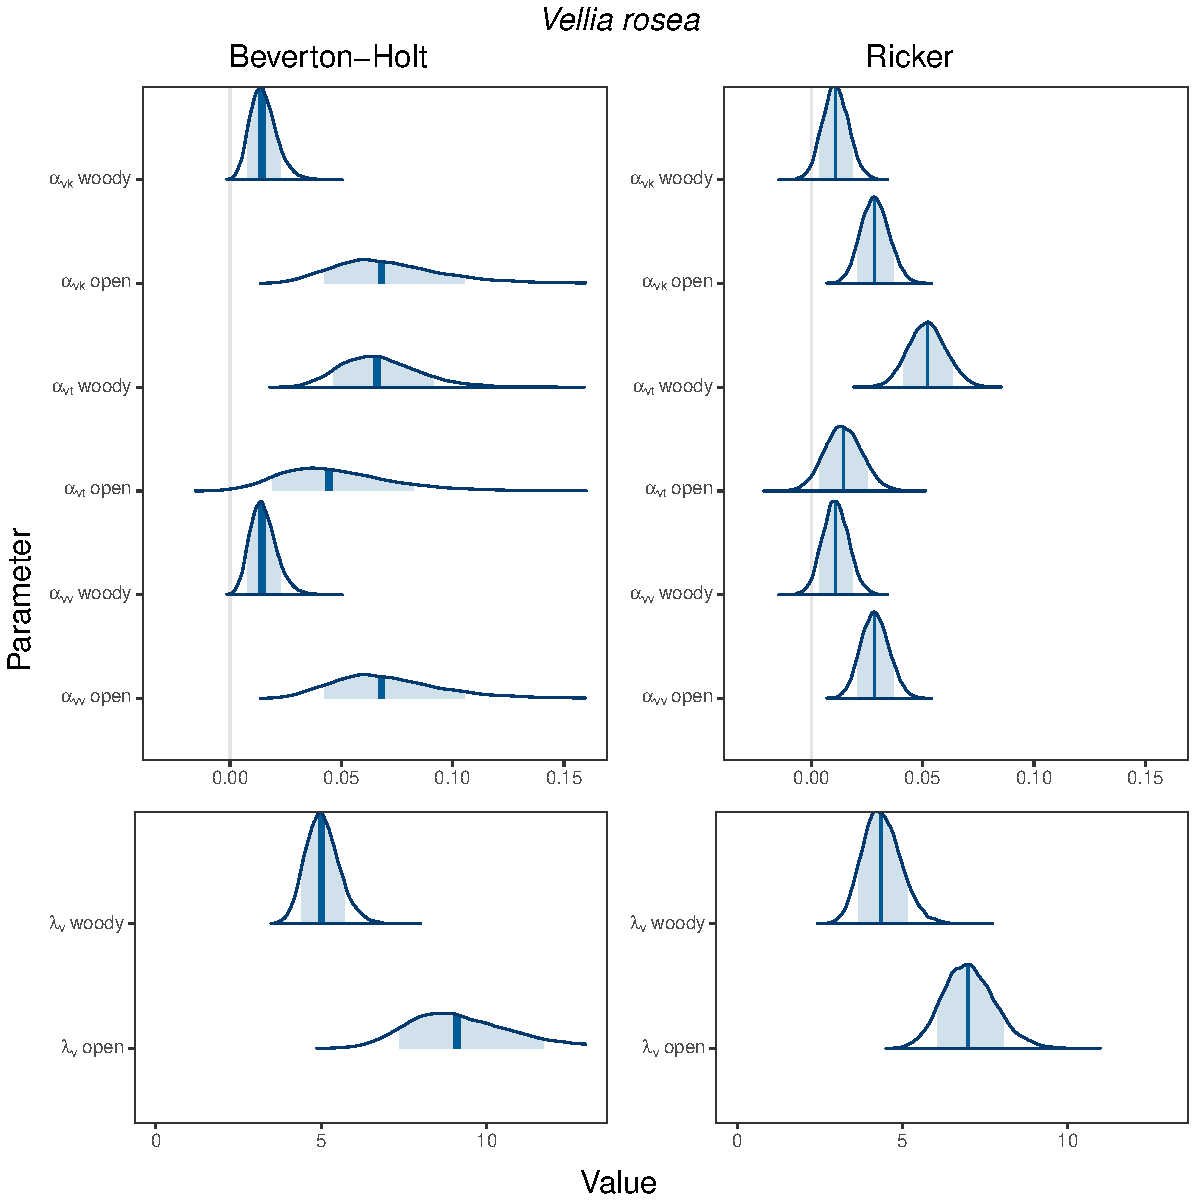
\includegraphics[width=1\textwidth]{figures/appendixB_fig1}}
  \caption[The posterior distributions of competition coefficients and intrinsic fecundity in the Beverton--Holt model and the Ricker model for \textit{Vellia rosea}.]{The posterior distributions of competition coefficients and intrinsic fecundity in the Beverton--Holt model and the Ricker model for \textit{Vellia rosea}. The subscript $v$ in parameter names denotes the species \textit{Vellia rosea}, while the subscript $t$ denotes the species \textit{Trachymene cyanopetala}, and the subscript $k$ other species that germinated in the system. Solid blue lines represent median estimates of parameter values, while shaded blue areas correspond to the 80\% probability mass of the posterior distribution of each parameter. Finally, we denote the environment where interactions took place to estimate parameter values with \textit{open} and \textit{woody}, as we do in \autoref{Bayesian_competition} }
  \label{fig:vero_dist}
\end{figure}

\clearpage

\begin{figure}[H]
  \centerline{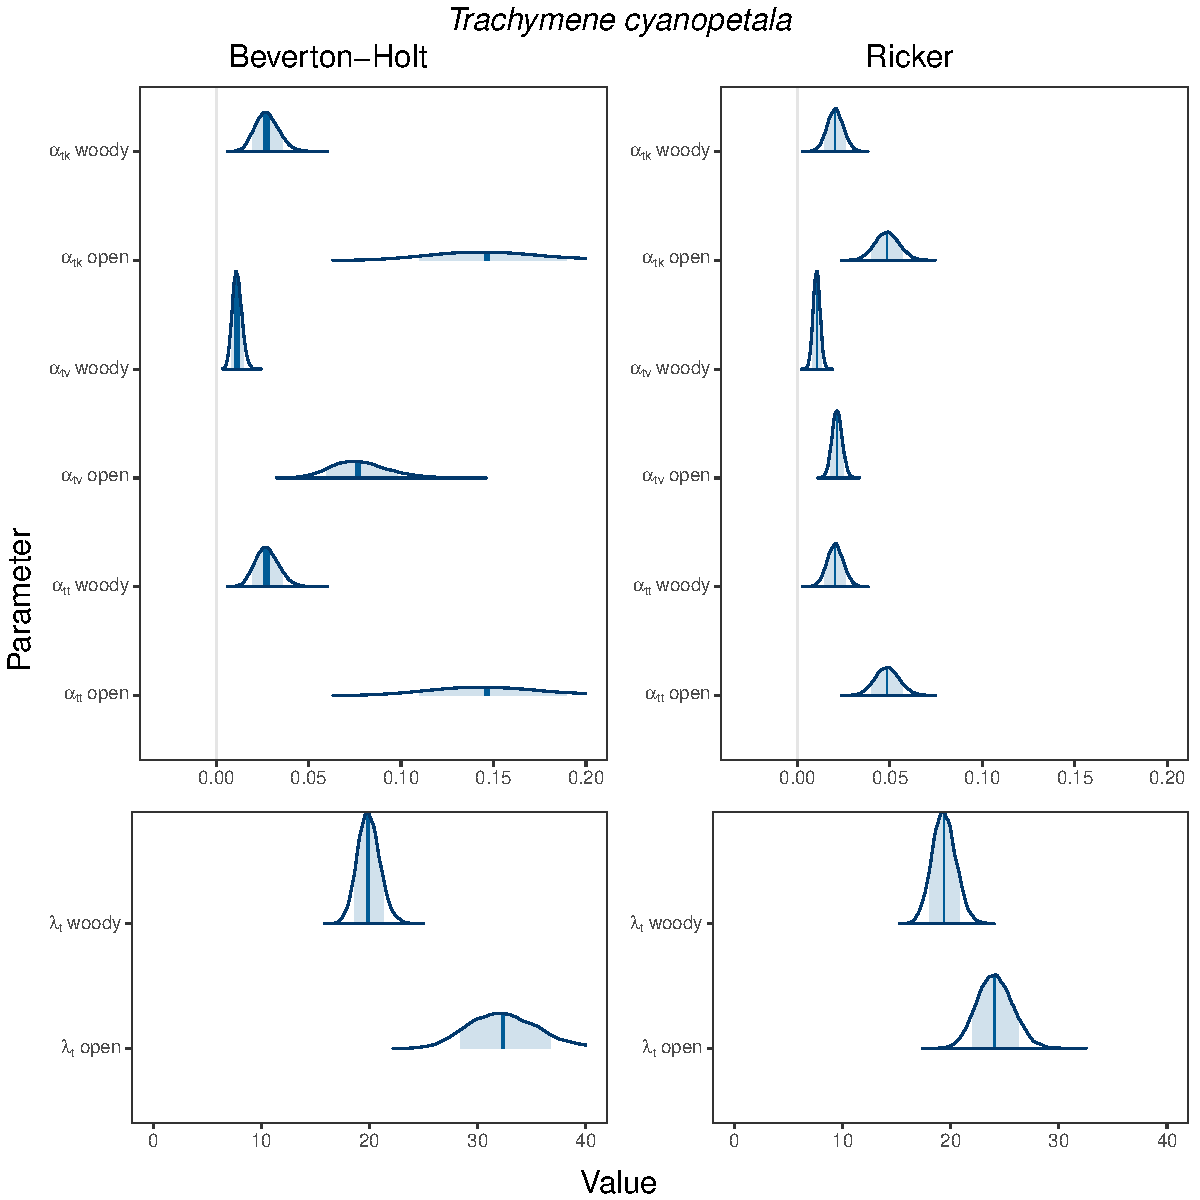
\includegraphics[width=1\textwidth]{figures/appendixB_fig2}}
  \caption[The posterior distributions of competition coefficients and intrinsic fecundity in the Beverton--Holt model and the Ricker model for \textit{Trachymene cyanopetala}]{  The posterior distributions of competition coefficients and intrinsic fecundity in the Beverton--Holt model and the Ricker model for \textit{Trachymene cyanopetala}. The subscript $v$ in parameter names denotes the species \textit{Vellia rosea}, while the subscript $t$ denotes the species \textit{Trachymene cyanopetala}, and the subscript $k$ other species that germinated in the system. Solid blue lines represent median estimates of parameter values, while shaded blue areas correspond to the 80\% probability mass of the posterior distribution of each parameter.  Finally, we denote the environment where interactions took place to estimate parameter values with \textit{open} and \textit{woody}, as we do in the \autoref{Bayesian_competition} }
  \label{fig:trcy_dist}
\end{figure}


\printbibliography
\end{refsection}
